\documentclass[10pt, letterpaper]{memoir}
\usepackage{HomeworkStyle}

\begin{document}
\begin{center}
	{\large Homework 13 -- Electronic Transitions}
	
	Due: Monday, April 2 \hspace{3em} Points: ${\dfrac{~}{~~60~~}}$
\end{center}

Name: \rule[-.1mm]{15em}{0.1pt}	
	
	\section*{Problem 1 (10 points)}
	Give the molecular term symbol for the lowest energy term arising from each electronic configuration. Be sure to use $_g$ or $_u$ subscripts to indicate inversion symmetry of the term where applicable.
	
	\noindent
	\begin{itemize}
		\item \ch{N2}: $\sigma_g^2{\sigma_u^*}^2\sigma_g^2\pi_u^4$ 
		
		\vspace{8em}
		\item \ch{O2}: $\sigma_g^2{\sigma_u^*}^2\sigma_g^2\pi_u^4{\pi_g^*}^2$ 
		
		\vspace{8em}
		\item \ch{C2^*}: $\sigma_g^2{\sigma_u^*}^2\sigma_g^2\pi_u^1{\pi_g^*}^1$ 
		
		\vspace{8em}
		\item \ch{CN}: $\sigma^2{\sigma^*}^2\sigma^2\pi^3$
		
		\vspace{8em}
		\item \ch{CO^*}:  $\sigma^2{\sigma^*}^2\sigma^2\pi^3{\pi^*}^1$
	\end{itemize}
	
	
	\newpage
	\section*{Problem 2 (10 points)}
	\begin{minipage}{0.5\linewidth}
		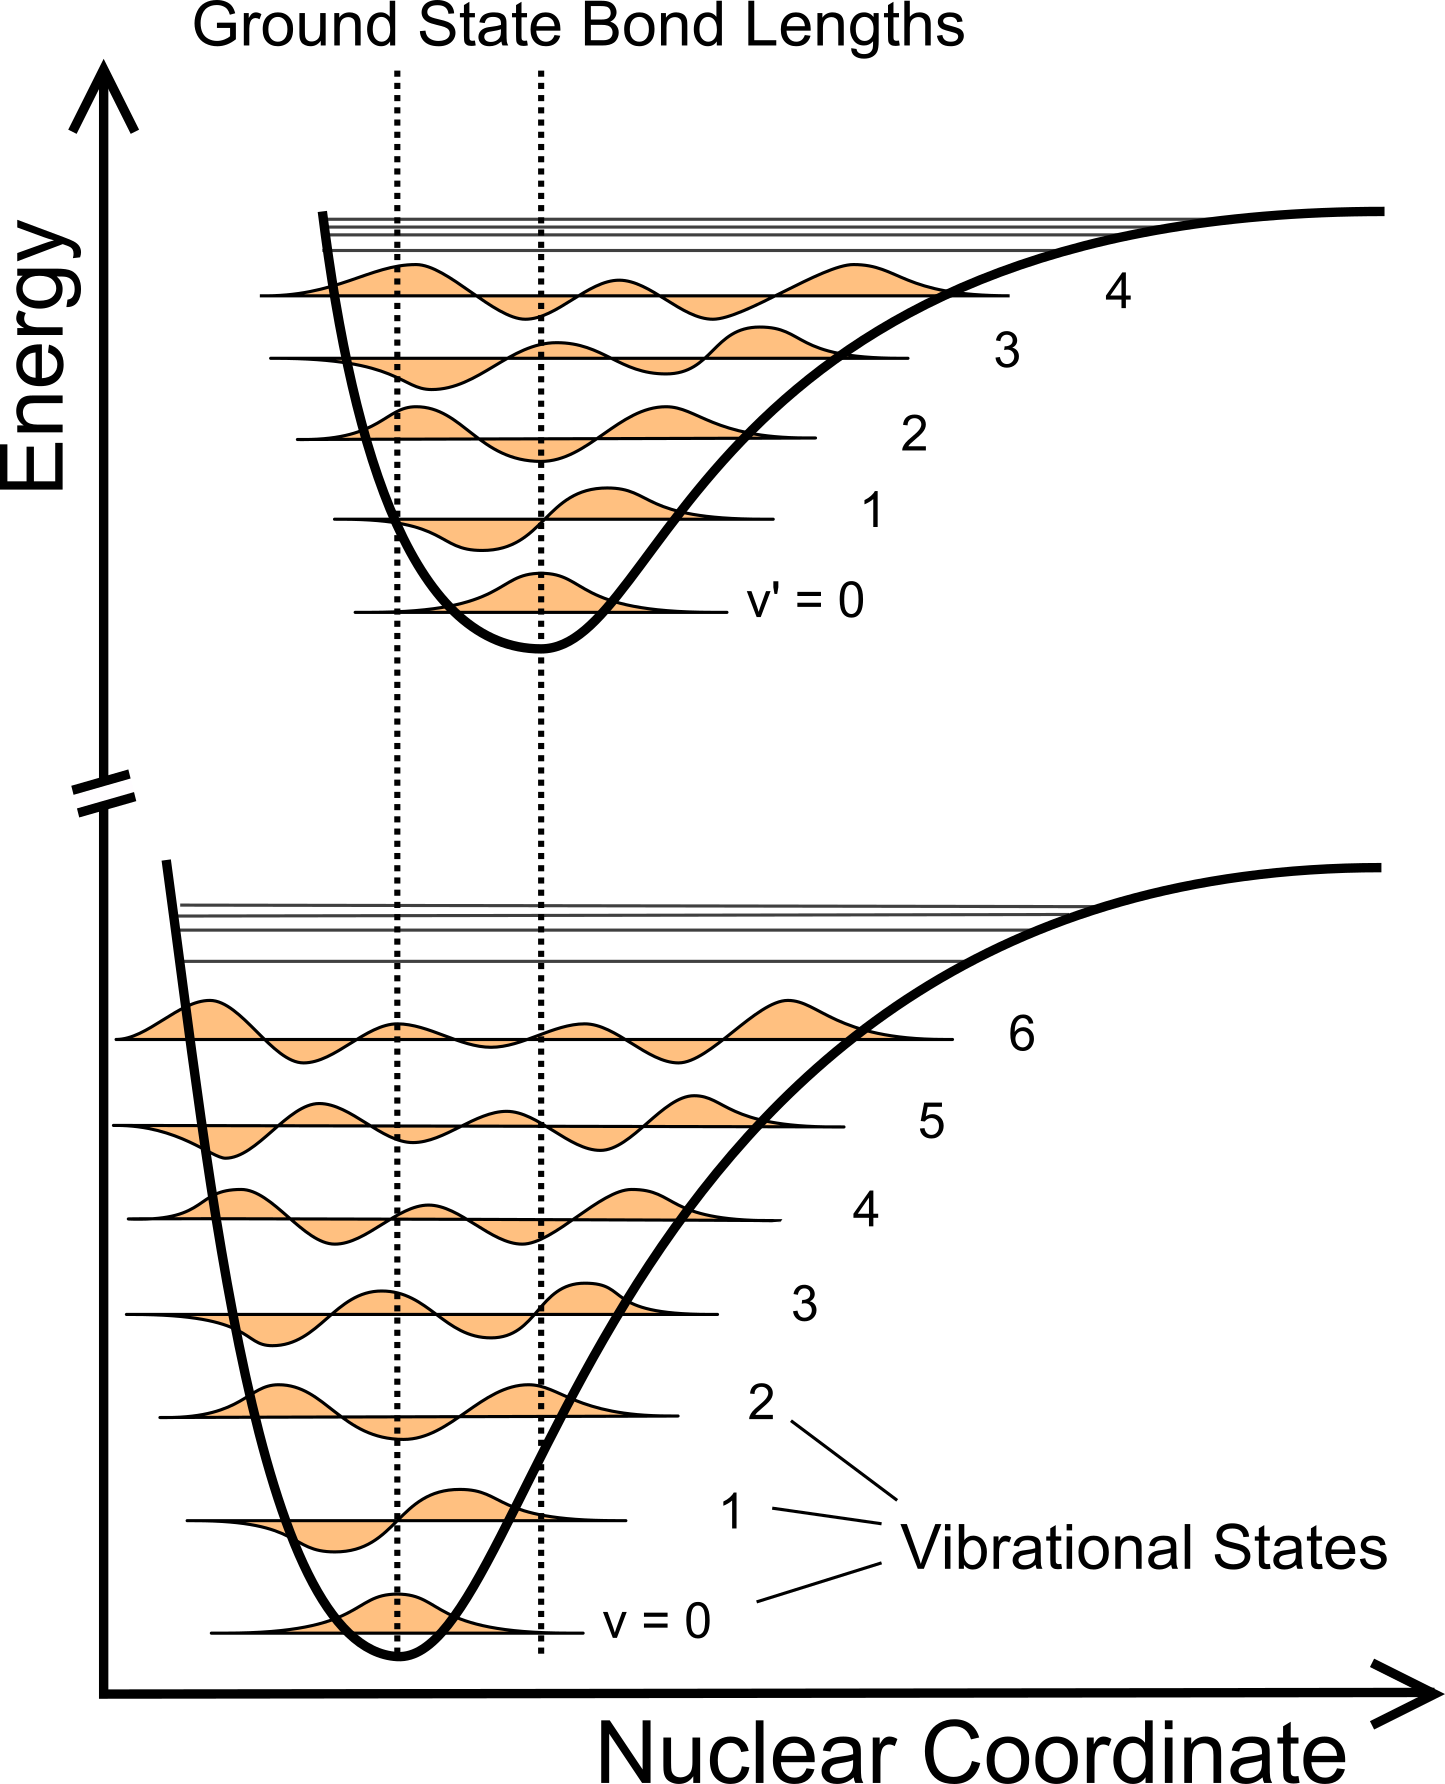
\includegraphics[width=\linewidth]{FC_Factors}
	\end{minipage}
	\begin{minipage}{0.5\linewidth}
		Shown at left are the first few vibrational states for the ground and excited electronic states in an electronic transition. For convenience, vertical dotted lines indicate the average bond lengths for the ground vibrational state in both electronic states.
		
		\noindent $\circ$ Suppose an absorption occurs from a hot band with $v=6$. Draw onto the diagram what is meant by a ``vertical transition,'' and predict which value of $v^\prime$ would be most prominent on the spectrum.
		
		\vspace{3em}
		\noindent$\circ$ Below, sketch how the absorption spectrum for this transition might look. Be sure to include vibrational structure. It need not be perfect, but should include features like the relative intensities and energies of the transitions.
		
		\noindent $\circ$ On the same axes, sketch how the fluorescence spectrum might look. Again, include all of the same features.
	\end{minipage}	

	\newpage
	\section*{Problem 3 (10 points)}	
	Tell whether the following transitions are allowed by selection rules.
	
	\begin{itemize}
		\item $^3\Pi_g \leftarrow ^3\Sigma_g^+$
		
		\vspace{2em}
		\item $^2\Sigma_g^+ \leftarrow ^2\Sigma_u^-$
		
		\vspace{2em}
		\item $^1\Pi \leftarrow ^3\Delta$
		
		\vspace{2em}
		\item $^1\Delta_g \leftarrow ^1\Sigma_u^-$
		
		\vspace{2em}
		\item $^2\Pi \leftarrow ^2\Sigma^+$
	\end{itemize}
	
	\section*{Problem 4 (10 points)}
	Shown below is an diagram of the transitions found in the electronic spectrum of the AID molecule. The digram was taken from a peer-reviewed article (W. Szajna, et al. Journal of Molecular Spectroscopy, 318 (2015) pp. 78-83).
	
	\noindent 	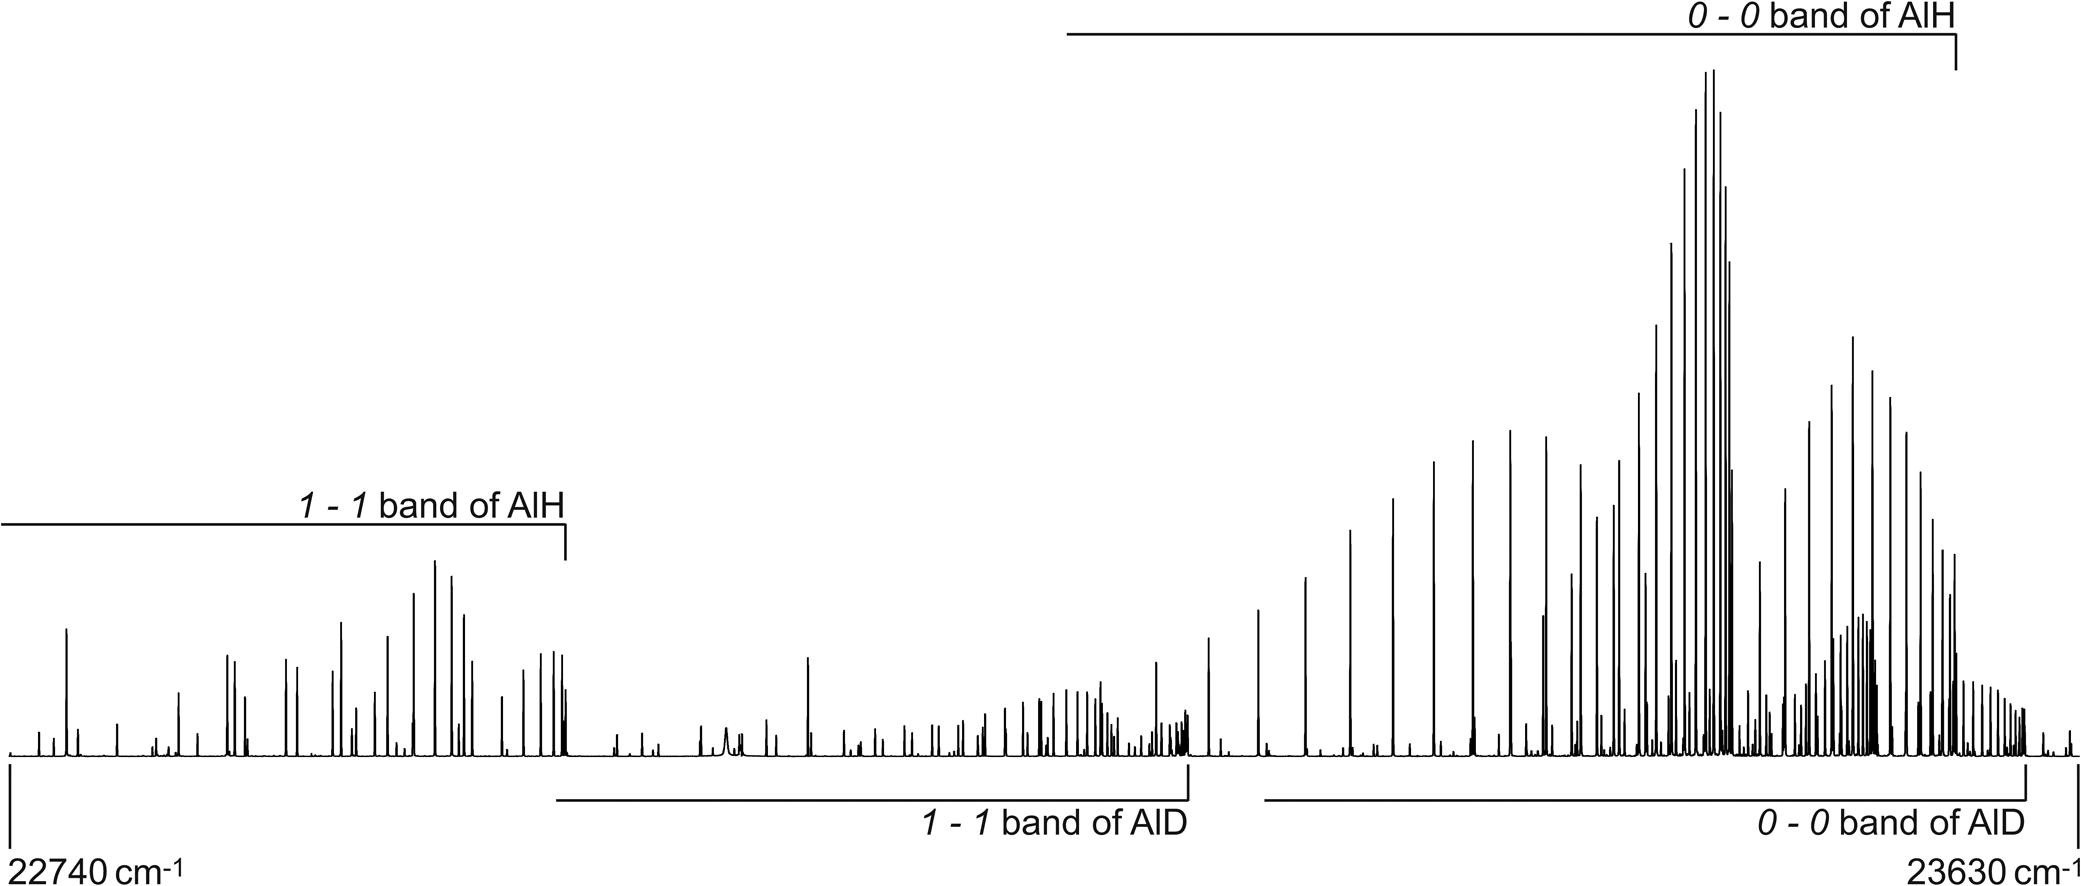
\includegraphics[width=\linewidth]{Band_Head}
	
	\noindent Does this electronic transition weaken or strengthen the AID bond? Briefly explain how you can tell. 

	\newpage
	\section*{Problem 5 (10 points)}
	Cobalt (III) cations can form metal complexes with a number of different ligands. Below is a table of the wavelengths at which a few of those complexes exhibit maximum absorbance:
	
	\begin{tabular}{c|c|c}
		Complex & $\lambda_{max}~(nm)$ & ~~~~$\Delta_O~(cm^{-1})$~~~~ \\ \midrule
		\ch{[CoF6]^{3-}} & $700$ & ~\\ & &\\
		\ch{[Co(H2O)6]^{3+}} & $600$ & ~\\ & &\\
		\ch{[Co(NH3)6]^{3+}} & $475$ & ~\\ & &\\
		\ch{[Co(CN)6]^{3-}} & $310$ & ~\\
	\end{tabular}
	
	\noindent $\circ$ Fill in the missing $\Delta_O$ column
	
	\noindent $\circ$ Draw a diagram of the energy levels involved in the transitions for the \ch{[Co(CN)6]^{3-}} and \ch{[CoF6]^{3-}} complexes. You may assume that the energy cost for pairing electrons in a single orbital lies somewhere between the energy of $700~nm$ and $310~nm$ light.
	
	\noindent $\circ$ Based on your diagrams, predict the magnetic properties of both the ground and excited states for both complexes.
	
	\vspace{10em}
	\section*{Problem 6 (10 points)}
	Below is the fluorescence spectrum for ``SYPRO Ruby,'' a fluorescent dye. You want to use the dye as a lasing medium, and place it in an optical cavity with length $L=0.25~m$. About how many longitudinal modes are possible for your laser (you may need to make some reasonable assumptions)?
	
	\noindent 	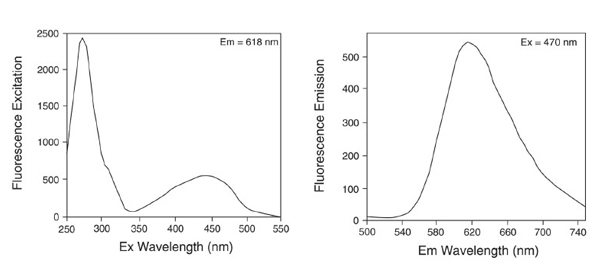
\includegraphics[trim = 300 0 0 0, clip, width=0.45\linewidth]{Dye_Fluorescence}
\end{document}
	